\chapter{Dealing with Uncertainty} 
\label{chapter:Benchmark Instances}

%%%%%%%%%%%%%%%%%%%%%%%%%%%%%%%%%%%%%%%%%%%%%%%%%%%%%%%%%%%%%%%%%%%%%% Section %%%%%%%%%%%%%%%%%%%%%%%%%%%%%%%%%%%%%%%%%%%%%%%

Following an initial analysis of the historical schedules and the discovery of significant room for optimisation, we now study the effects that the addition of an \textbf{uncertainty component} will have on our schedules.

\vspace{\baselineskip}
\noindent
The chapter begins by outlining the reasoning behind our wish to examine the concept of uncertainty. Section \ref{section: Generating Uncertainty} begins the study by discussing the procedures followed to generate the uncertainty components. Section \ref{section: effect of uncertainty} continues that discussion by analysing the effect the uncertainty components have on our previously optimally generated schedules. It focuses on the robustness of those optimal schedules. Finally, Section \ref{section: Methodologies} studies two new methodologies that will hopefully enhance the robustness of our proposed schedule, and compares every optimal schedule that we have generated to determine the most robust, with respect to the uncertainty components.

%%%%%%%%%%%%%%%%%%%%%%%%%%%%%%%%%%%%%%%%%%%%%%%%%%%%%%%%%%%%%%%%%%%%%% Section %%%%%%%%%%%%%%%%%%%%%%%%%%%%%%%%%%%%%%%%%%%%%%%

\vspace{\baselineskip}
\noindent
 Our study on uncertainty begins by considering the optimal schedule from the Makespan Scheduling Section \ref{section:Makespan Scheduling-content} of Chapter \ref{chapter: 2-Evaluating Royal Mail Historical Data}. In particular, henceforth we call the \textbf{Makespan optimised} schedule from the Historical dataset our \textbf{nominal} instance. In essence, it represents what we would like to take place at the MC for the majority of the time. However, for the purposes of this uncertainty study we want to investigate the degree to which this optimal schedule is \textbf{robust} with respect to various degrees of \textbf{uncertainty}. The purpose of studying this, is to ensure that the schedules generated from our optimisation models will withstand random perturbations that simulate what might occur on a given day at Royal Mail. We argue that robustness of a schedule is dependent upon two optimality criteria. When comparing two schedules, we can characterise as more robust the schedule that achieves the lowest makespan value \cite{DBLP:approximatingbounded} or the least amount of duties that end up overrunning a maximum duty threshold, defined below. In cases that one schedule performs better in one of the criteria and the other outperforms it in the other criterion, it is left to the scheduler's judgement to determine which schedule is more robust depending on the magnitude of the out-performance in the respective criterion.

%%%%%%%%%%%%%%%%%%%%%%%%%%%%%%%%%%%%%%%%%%%%%%%%%%%%%%%%%%%%%%%%%%%%%% Figure %%%%%%%%%%%%%%%%%%%%%%%%%%%%%%%%%%%%%%%%%%%%%%%

\begin{figure}
    \centering
    \begin{tikzpicture}[%
        every node/.style={
            font=\scriptsize,
            % Better alignment, see https://tex.stackexchange.com/questions/315075
            text height=1ex,
            text depth=.25ex,
        },
    ]
    % draw horizontal line   
    \draw[->] (1,0) -- (8.5,0);
    
    % draw vertical lines
    \foreach \x in {1,...,8}{
        \draw (\x cm,3pt) -- (\x cm,0pt);
    }
    
    % place axis labels
    \node[anchor=north] at (3,0) {$t-2$};
    \node[anchor=north] at (4,0) {$t-1$};
    \node[anchor=north] at (5,0) {$t$};
    \node[anchor=north] at (6,0) {$t+1$};
    \node[anchor=north] at (7,0) {$t+2$};
    \node[anchor=north] at (8.5,0) {time};
    
    % Bar for Block1
    %\draw[fill=myLightGray] (1,0.25) rectangle (2,0.6);
    \fill[myLightGray] (1,0.25) rectangle (2,0.6);
    \fill[myLightGray] (2,0.25) rectangle (3,0.6);
    \fill[myLightGray] (3,0.25) rectangle (4,0.6);
    \fill[myLightGray] (4,0.25) rectangle (5,0.6);
    \draw[myRed,dashed,thick,-latex] (5.05,0.425) -- (7.05,0.425);
    \draw[myRed,dashed,thick,-latex] (5.05,0.425) -- (3,0.425);
    
    % Bar for Block2
    \fill[myLightGray] (1,1) rectangle (3,1.35);
    \fill[myLightGray] (3,1) rectangle (4,1.35);
    \fill[myLightGray] (4,1) rectangle (5,1.35);
    \fill[myLightGray] (5,1) rectangle (5.4,1.35);
    \draw[myGreen,dashed,thick,-latex] (5.405,1.175) -- (7.05,1.175);
    \draw[myGreen,dashed,thick,-latex] (5.405,1.175) -- (3.8,1.175);
    
    % Bar for Block3
    \fill[myLightGray] (1,1.75) rectangle (3,2.1);
    \fill[myLightGray] (3,1.75) rectangle (4,2.1);
    \fill[myLightGray] (4,1.75) rectangle (5,2.1);
    \fill[myLightGray] (5,1.75) rectangle (5.8,2.1);
    \draw[myBlue,dashed,thick,-latex] (5.805,1.925) -- (7.05,1.925);
    \draw[myBlue,dashed,thick,-latex] (5.805,1.925) -- (4.6,1.925);
    
    % draw curly braces and add their labels
    \draw[decorate,decoration={brace,amplitude=5pt}] (3,0.45) -- (5,0.45)
        node[anchor=south,midway,above=4pt] {$U$:$-$50\%};
    \draw[decorate,decoration={brace,amplitude=5pt}] (5,0.45) -- (7,0.45)
        node[anchor=south,midway,above=4pt] {$U$:$+$50\%};  
        
    \draw[decorate,decoration={brace,amplitude=5pt}] (3.8,1.175) -- (5.405,1.175)
        node[anchor=south,midway,above=4pt] {$U$:$-$40\%};
    \draw[decorate,decoration={brace,amplitude=5pt}] (5.405,1.175) -- (7.05,1.175)
        node[anchor=south,midway,above=4pt] {$U$:$+$40\%};   
        
    \draw[decorate,decoration={brace,amplitude=5pt}] (4.6,1.925) -- (5.805,1.925) 
        node[anchor=south,midway,above=4pt] {$U$:$-$30\%};
    \draw[decorate,decoration={brace,amplitude=5pt}] (5.805,1.925)  -- (7.05,1.925)
        node[anchor=south,midway,above=4pt] {$U$:$+$30\%};       
        
    % Place the label inside block:
    \node [darkgray] at (+0.5,0.425) {$Block_3$};
    \node [darkgray] at (+0.5,1.175) {$Block_2$};
    \node [darkgray] at (+0.5,1.925) {$Block_1$};
    %\node [centre,darkgray] at (+6,0.7) {};
    %\node [centre,darkgray] at (+4,0.7) {};
    
    \end{tikzpicture}
    \caption{The effect of the application of box uncertainty sets of different magnitudes on the duration of blocks.}
    \label{fig:Generating Uncertainty}
\end{figure}

\section{Uncertainty Generation}
\label{section: Generating Uncertainty}
We generate \textit{disturbed} instances by using the nominal instance as our foundation, to which we then apply uncertainty components of various magnitudes. The uncertainty components are applied onto each schedule's blocks, which we subsequently will attempt to fit inside the duties. We begin by applying \textbf{box uncertainty sets} of magnitudes $U:$ $\pm30\%$,$\pm40\%$,$\pm50\%$ respectively. As seen for example on Figure \ref{fig:Generating Uncertainty}, when we apply an uncertainty component of magnitude $U$: $\pm30\%$, each block's \textit{processing time} $p_j$ can randomly \textbf{shrink} or \textbf{expand} by up to a maximum of 30\%, equivalently for uncertainty sets of other magnitudes. 

\todo{add a thing like schedule apply uncertainty recovered}

\vspace{\baselineskip}
\noindent
In generating the first set of samples, we created ten disturbed instances per uncertainty set, a total of 30. We chose to showcase the \textbf{most disturbed} instances in Table \ref{table:Applying Uncertainty Set on Nominal}. We measure the disturbance of the uncertainty set on the instance by examining the degree to which the \texttt{Total Time} of the instance has increased or decreased. Hence, for each uncertainty set we present the two instances for which we observed the largest increase, and decrease of the \texttt{Total Time} away from the nominal instance's \texttt{Total Time} benchmark. We henceforth refer to each group as \texttt{reduced} and \texttt{augmented}, for reduced and increased \textit{Total time} respectively \cite{DBLP:journals/corr/abs-1805-03437}. 

\vspace{\baselineskip}
\noindent
The thought process behind choosing the most disturbed instances per uncertainty set, is based on the idea that less disturbed instances will achieve levels of performance in between these two extremes when optimised, hence we can approximate their performance by using those two boundary cases for our analysis. 

%%%%%%%%%%%%%%%%%%%%%%%%%%%%%%%%%%%%%%%%%%%%%%%%%%%%%%%%%%%%%%%%%%%%%%%%%%%%%%% Table %%%%%%%%%%%%%%%%%%%%%%%%%%%%%%%%%%%%%%%%%%%%%%%%%%%%%%%%%%%%%%%%%%%%%%%%%%%%%%

\begin{table}[t]
\small
    \centering 
    \begin{tabular}{|c|c|c|c|c|}
        \hline
        \textbf{Instance} & \textbf{Total Time} & \multicolumn{3}{|c|}{ \textbf{Atomic Blocks} \textbf{(}$\pmb{p_j}$\textbf{)}} \\
        \hline
         \multicolumn{2}{|c|}{ }  & \texttt{Average} &  \texttt{Minimum} & \texttt{Maximum} \\
        \hline
        Nominal & 1,435:22  & 03:05 & 00:40 & 08:25 \\
        \hline
        \multirow{2}{*}{$U$: $\pm30\%$} & 1,416:36 & 03:03 & 00:30 & 10:00 \\
        \cline{2-5}
         & 1,446:14 & 03:07 & 00:29 & 10:12  \\
        \hline
        \multirow{2}{*}{$U$: $\pm40\%$} & 1,406:34 & 03:02 & 00:30 & 10:55  \\
        \cline{2-5}
         & 1,439:28 & 03:06 & 00:32 & 11:26 \\
        \hline
        \multirow{2}{*}{$U$: $\pm50\%$} & 1,391:17 & 03:00 & 00:23 & 10:44  \\
        \cline{2-5}
         & 1,454:18 & 03:08 & 00:20 & 10:52  \\
        \hline
    \end{tabular}%
    \medbreak
    \caption{Table showing the overall labor time and other characteristic values of atomic blocks from the two \textbf{most disturbed} (\texttt{reduced}, \texttt{augmented}) instances for each uncertainty set in (HH:mm).}
    \label{table:Applying Uncertainty Set on Nominal}
\end{table}

%%%%%%%%%%%%%%%%%%%%%%%%%%%%%%%%%%%%%%%%%%%%%%%%%%%%%%%%%%%%%%%%%%%%%% sub-Section %%%%%%%%%%%%%%%%%%%%%%%%%%%%%%%%%%%%%%%%%%%%%%%

\subsection*{Analysis of the Generated Instances}
\label{subsection: Analysis of  Disturbed Instances}
It is evident in Table \ref{table:Applying Uncertainty Set on Nominal} that the application of the uncertainty components will likely decrease the optimal nature of the nominal schedule, with respect to the makespan. This can be deduced from the fact that the nominal instance contains around 1,435 labour hours whereas in some cases the perturbed instances end up having to schedule more labour hours. By definition the more time that requires scheduling means the tougher for the optimisation solver to fit all blocks in a schedule with a reduced makespan. Hence, this first observation already hints to schedules with generally increased makespans for the disturbed instances. 

\vspace{\baselineskip}
\noindent
Moreover, as the magnitude of the uncertainty set is increased, we can see that the extremities as far as the durations of the blocks tend to increase accordingly. The increase in the duration of the longest lasting blocks will most likely result in a less robust schedule. Assuming our disturbed instance is \textbf{maximally disturbed} as those in Table \ref{table:Applying Uncertainty Set on Nominal}, we can see that there exist blocks that have a \textit{processing time} $p_j$ that surpasses the maximum $p_j$ observed in the nominal instance. As we saw in Section \ref{section:Makespan Scheduling-content} the maximum $p_j$ of 08:25 in the nominal instance also coincides with the nominal schedule's \textit{makespan}. Hence, the disturbed blocks with \texttt{Maximum} ($p_j$)\footnote{Observed in the final column of Table \ref{table:Applying Uncertainty Set on Nominal}} have durations larger than the nominal instance's makespan. Consequently, it is inevitable, even if the solver encloses only those particular blocks by themselves in one duty, to expect an increased makespan for the disturbed instances over the nominal instance. 

\vspace{\baselineskip}
\noindent
On the contrary, looking at the other end of the spectrum we can see that the \texttt{Minimum} ($p_j$) involves blocks with reduced \textit{processing times}. The blocks with shorter lasting durations are potentially going to be helpful in ensuring the uniformity of the optimised schedule since the solver can utilise them as a final buffer to be used in filling any non-utilised idle time at the end of a duty. In simple terms, the blocks with minimal processing times allow the solver greater flexibility in putting the duties together.

%%%%%%%%%%%%%%%%%%%%%%%%%%%%%%%%%%%%%%%%%%%%%%%%%%%%%%%%%%%%%%%%%%%%%% Section %%%%%%%%%%%%%%%%%%%%%%%%%%%%%%%%%%%%%%%%%%%%%%%

\section{Evaluating the Effect of Uncertainty}
\label{section: effect of uncertainty}
Having generated this new set of instances of the problem, our goal is to detect the effects theses various \textbf{degrees of uncertainty} have on the optimality of the nominal instance. We hypothesise that there exists a maximum duty threshold \textit{L} of 8 hours and 25 minutes, that should ideally not be exceeded by any duty under the application of uncertainty. Choosing the two most disturbed instances of Table \ref{table:Applying Uncertainty Set on Nominal} for each uncertainty set, we would like to measure the degree to which the optimised nominal schedule with makespan equal to \textit{L}, is \textbf{disturbed} for each set. The degree of the disturbance is evaluated by measuring the number of duties that overrun this \textit{L} plus a 15 minute interval, i.e. a \textbf{delay of a quarter of an hour}. We refer to this length of time as \textit{L'}. The purpose of this experiment is to gain an insight into the level of robustness of the nominal schedule, with respect to uncertainty. We pass each instance $D$ to the optimisation solver and by applying the \textbf{Makespan Scheduling} formulation of Section \ref{section:Makespan Scheduling-content}, we observe the effects in Table \ref{table:Uncertainty Schedules} and Figure \ref{fig: Uncertainty Sets Effects.}.

%%%%%%%%%%%%%%%%%%%%%%%%%%%%%%%%%%%%%%%%%%%%%%%%%%%%%%% Double Figure %%%%%%%%%%%%%%%%%%%%%%%%%%%%%%%%%%%%%%%%%%%%%%%%%%%%%%%%%%%%%%%%%%%%%%%%%%%

\begin{figure}%
    \centering
    \subfloat[Maximally disturbed instances with a \textbf{decrease} in overall labor time (\texttt{reduced}).]{%\begin{center}
    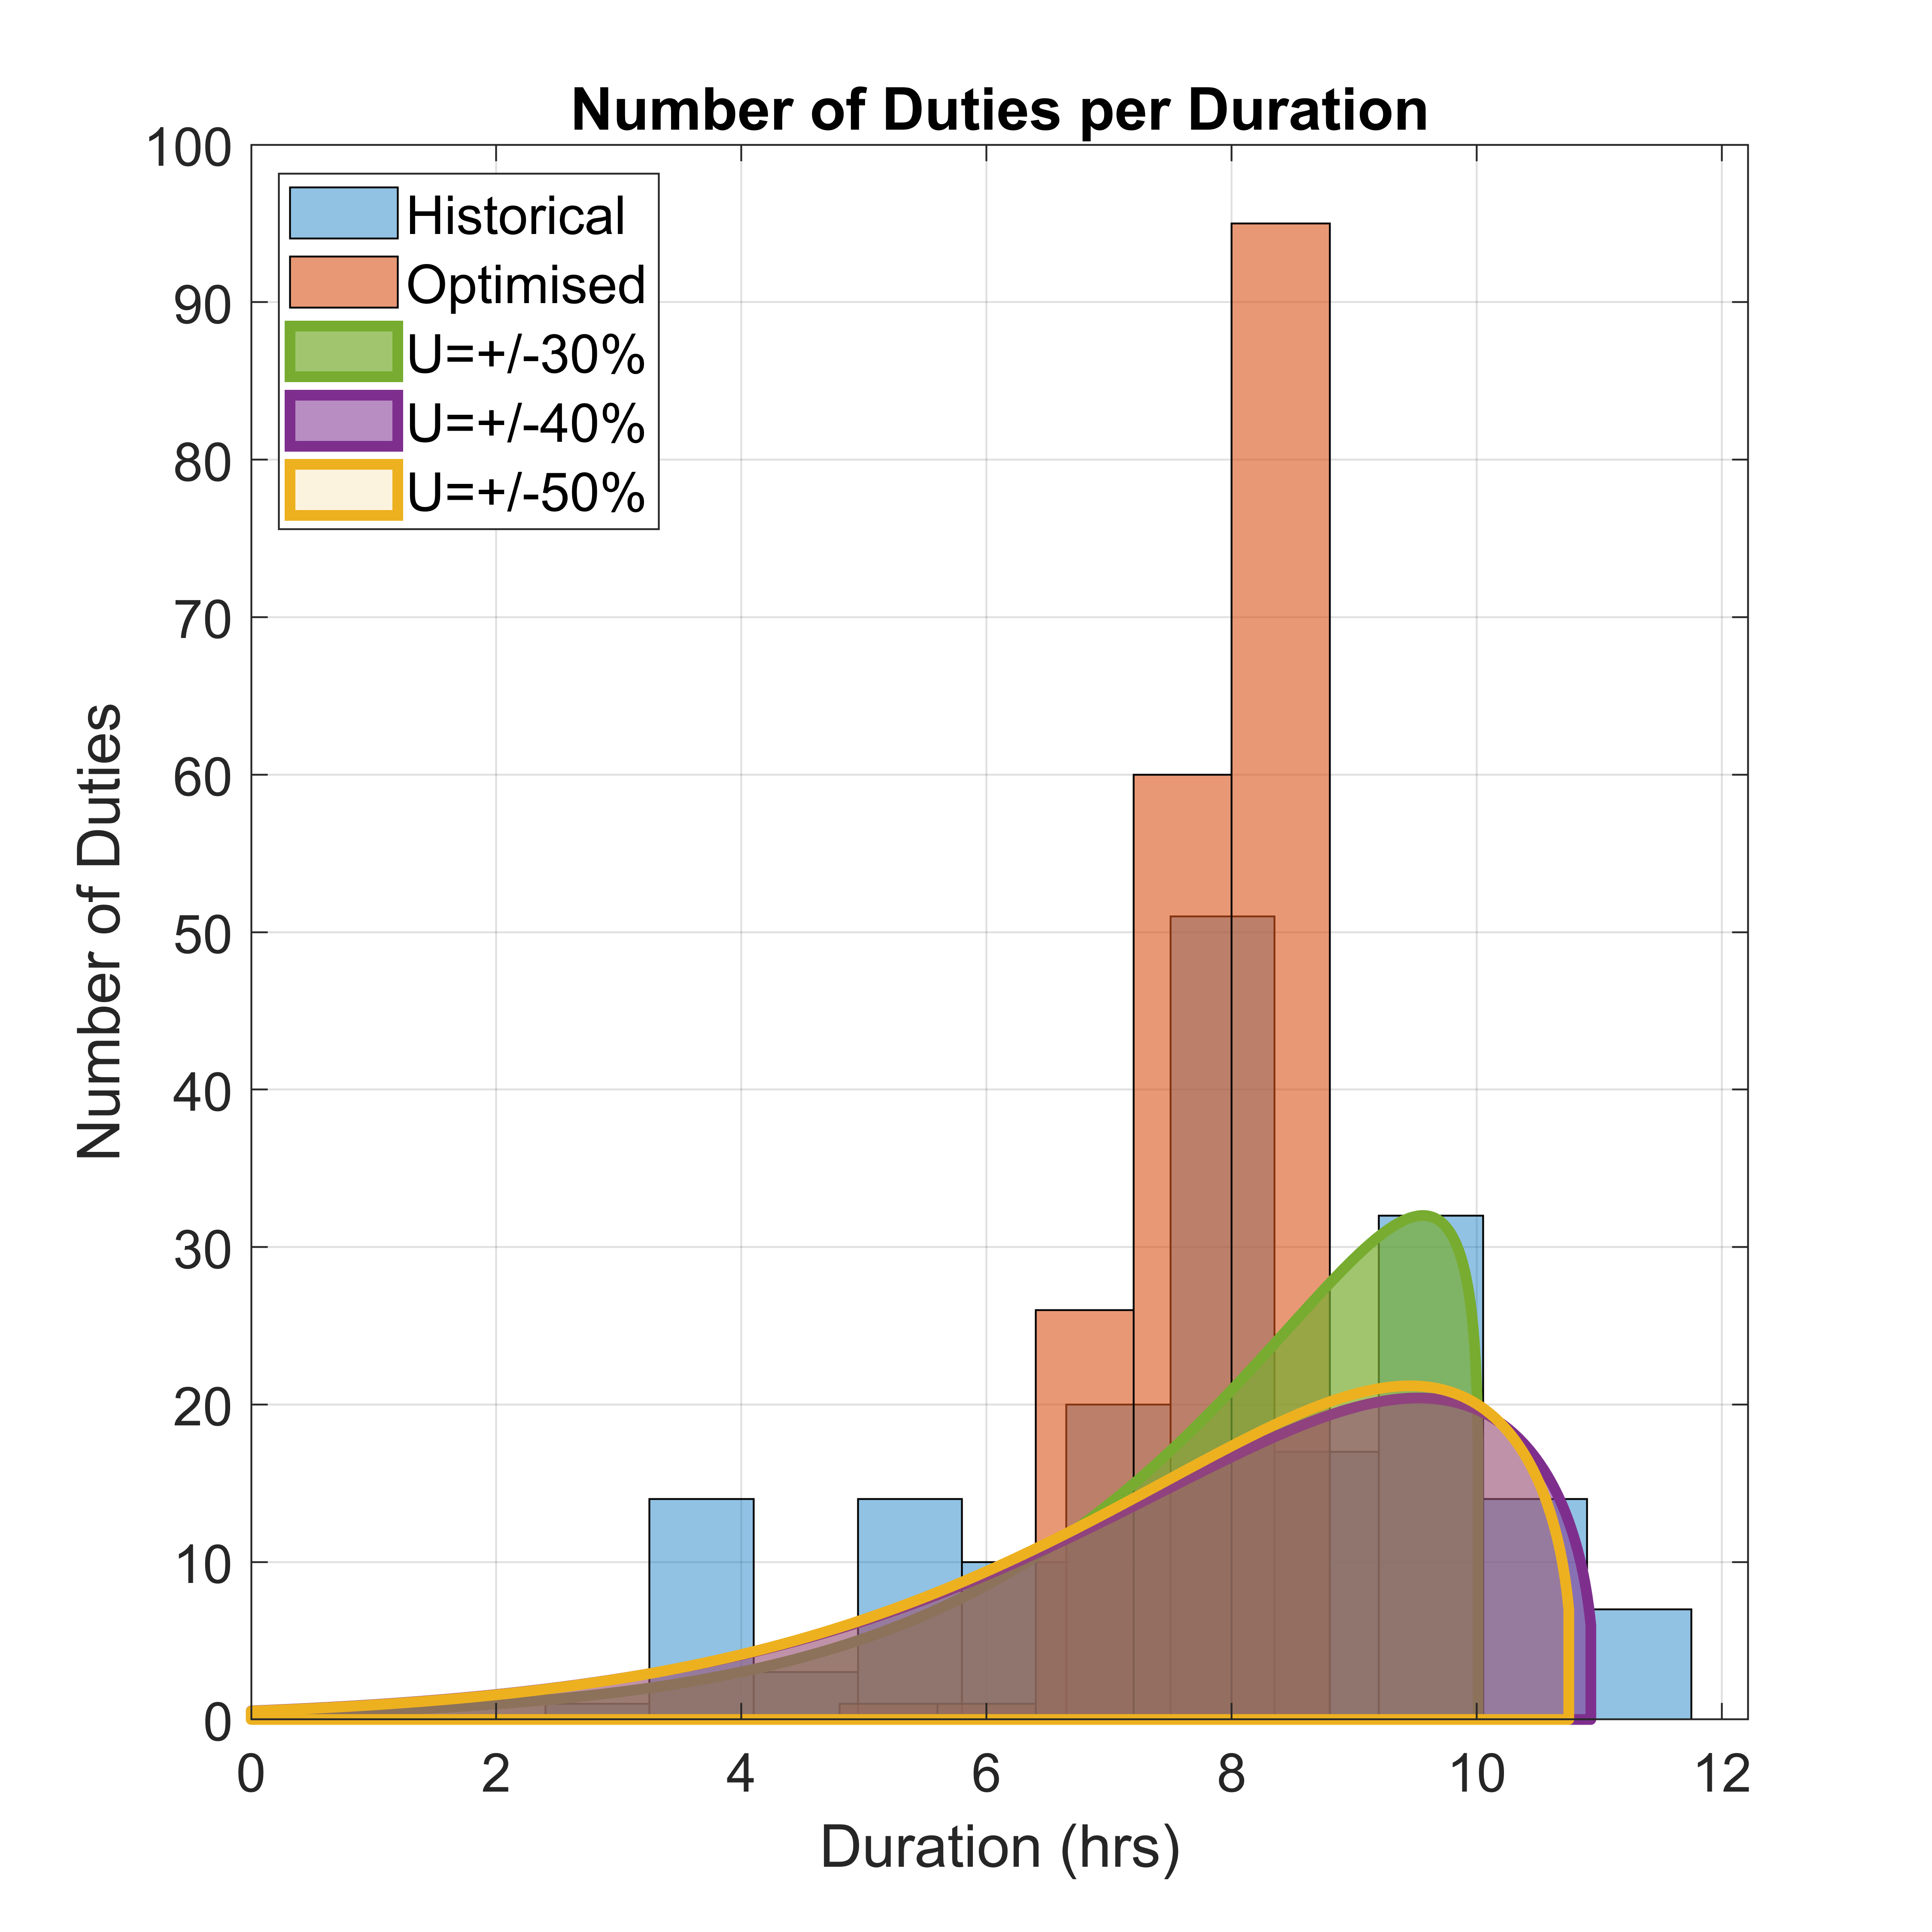
\includegraphics[width=0.46\linewidth]{[3] - chapter/Comparison_Of_Uncertainty_Sets_min.png}
    }%\end{center}}%end of picture #2
    \qquad
    %picture #2
    \centering
    \subfloat[Maximally disturbed instances with an \textbf{increase} in overall labor time (\texttt{augmented}).]{%\begin{center}
    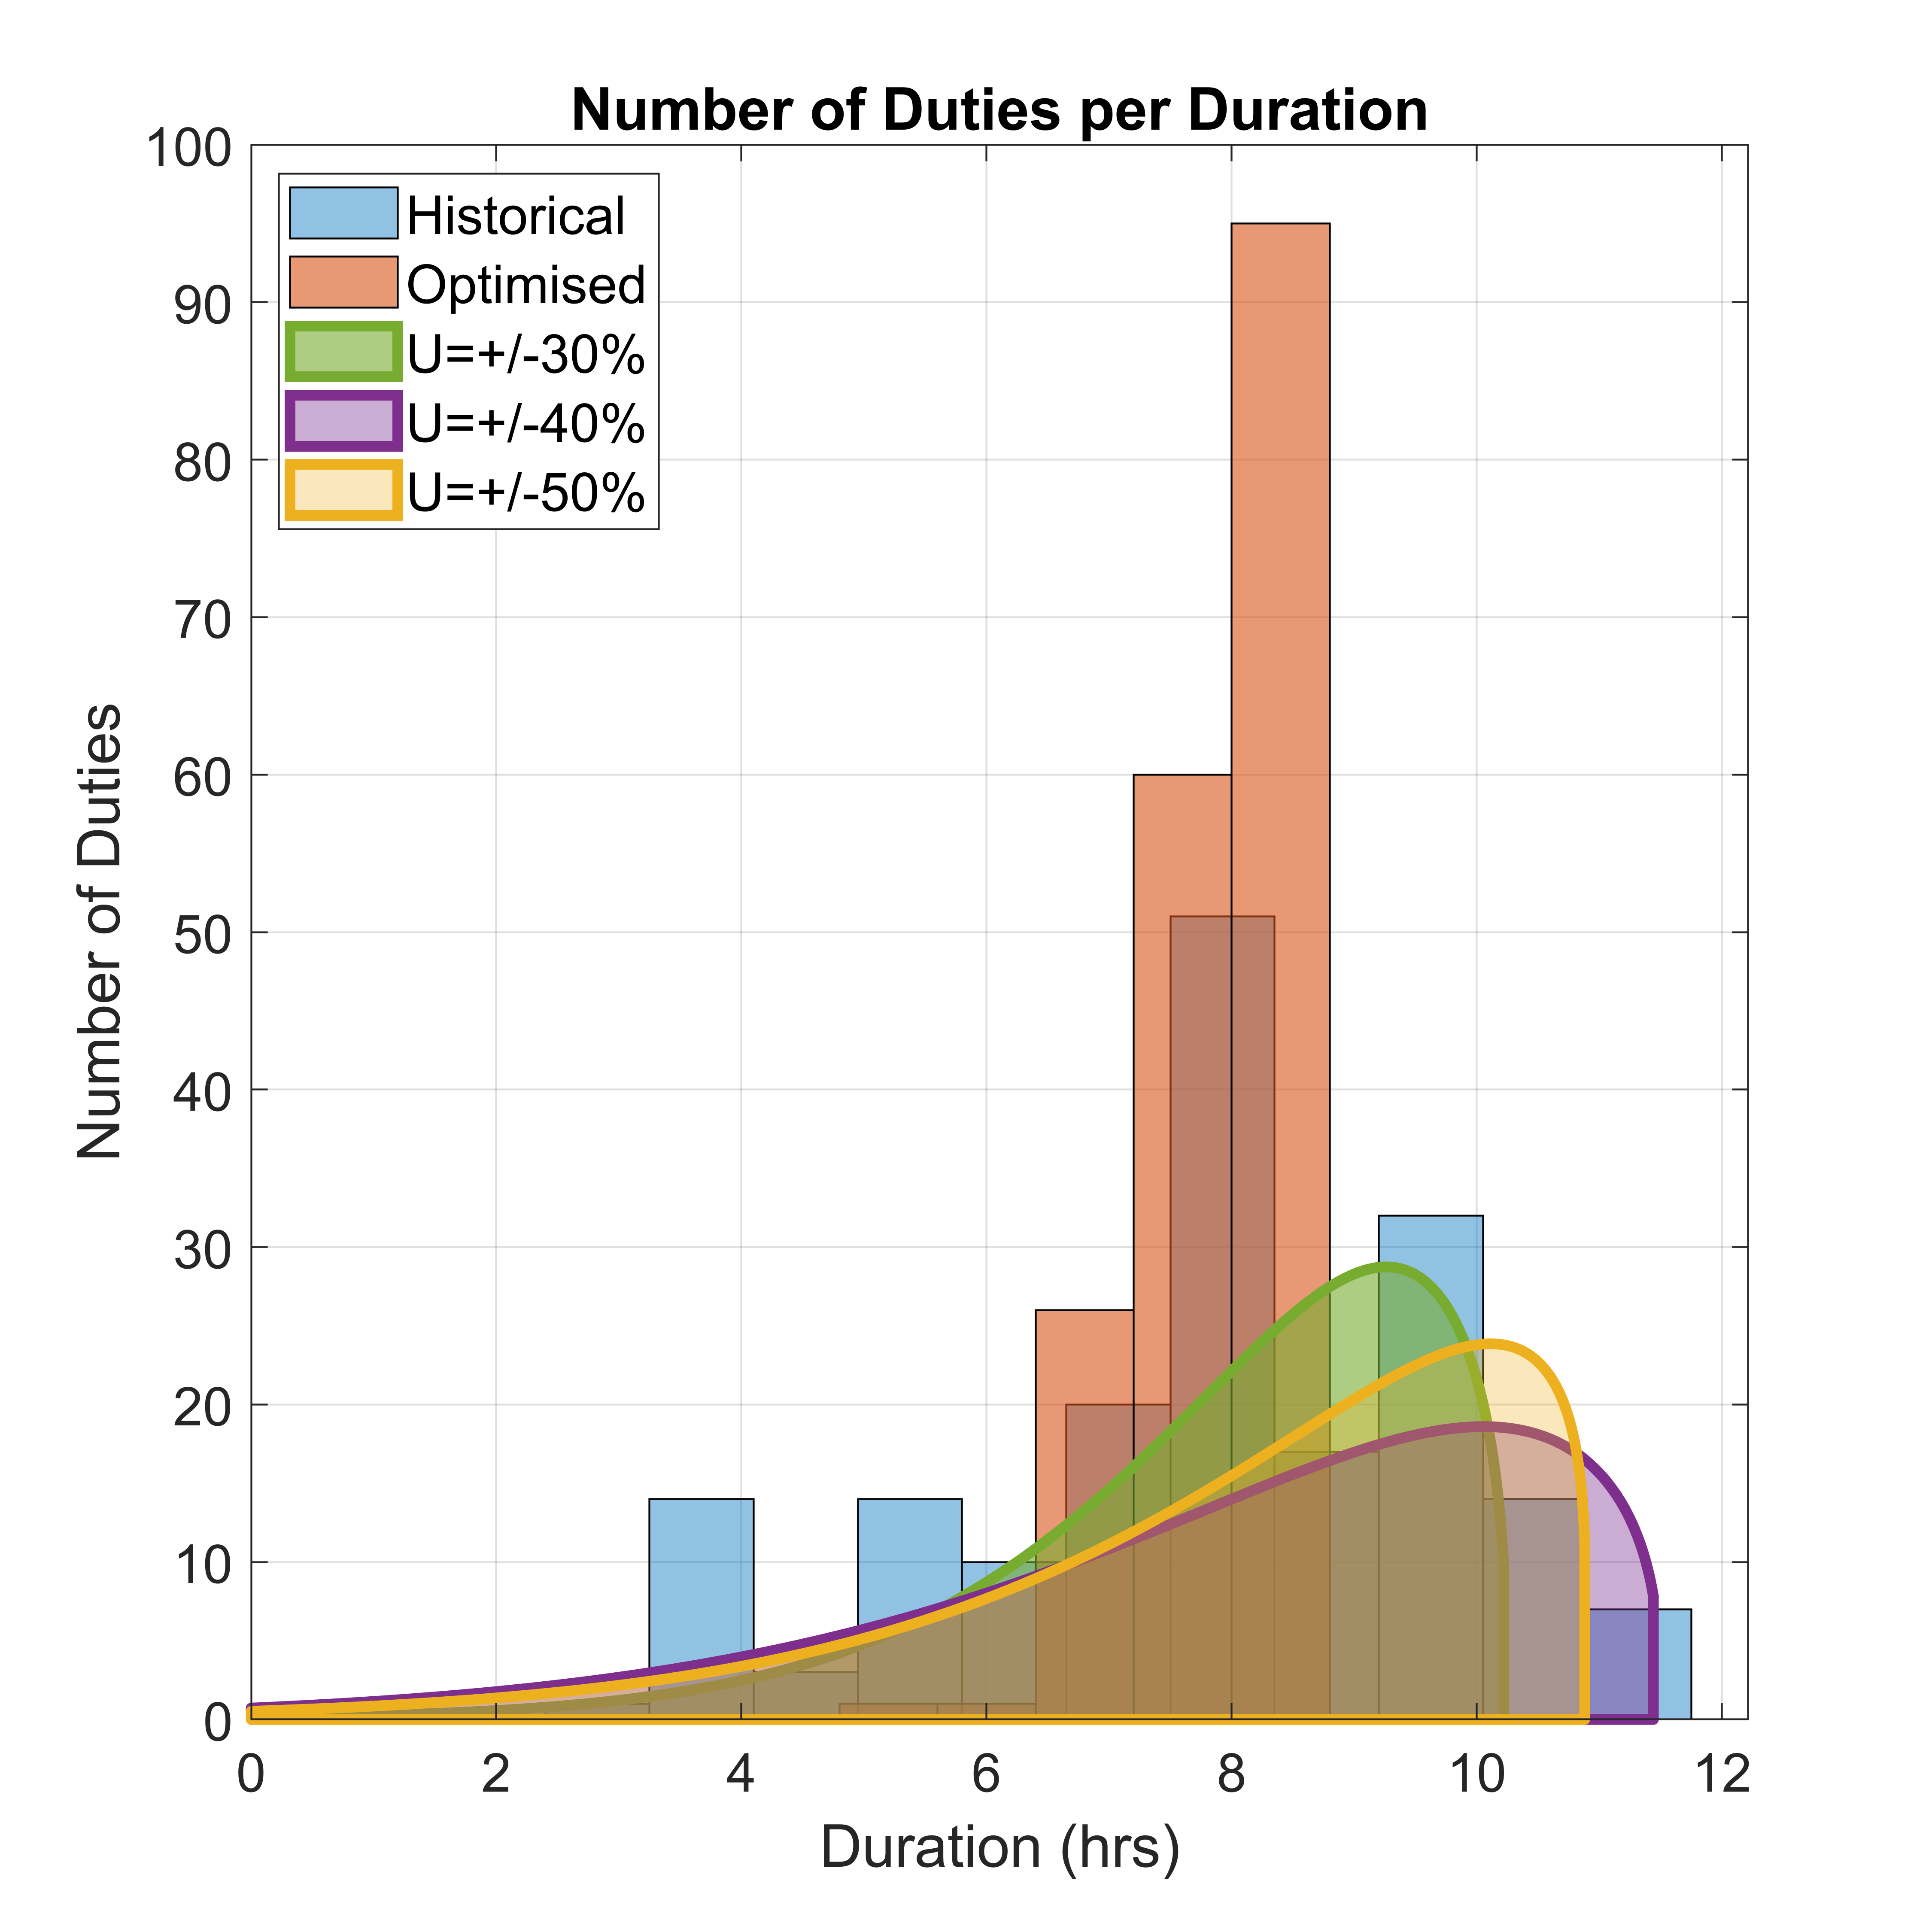
\includegraphics[width=0.46\linewidth]{[3] - chapter/Comparison_Of_Uncertainty_Sets_max.png}
    }%\end{center}}%picture #1
    \caption{The histograms provide an overview of the effects of various levels of uncertainty set on $Duty$ lengths.}
    \label{fig: Uncertainty Sets Effects.}
\end{figure}

%%%%%%%%%%%%%%%%%%%%%%%%%%%%%%%%%%%%%%%%%%%%%%%%%%%%%%%%%%%%%%%%%%%%%% Table %%%%%%%%%%%%%%%%%%%%%%%%%%%%%%%%%%%%%%%%%%%%%%%

\begin{table}[b]
\small
    \centering 
    \begin{tabular}{|c|c|c|c|c|}
        \hline
        \textbf{Schedule} & \textbf{Total Time} & \multicolumn{3}{|c|}{ \textbf{Duties (HH:mm)}} \\
        \hline
        \multicolumn{2}{|c|}{ }  & \texttt{Makespan} & \texttt{Minimum} & \texttt{Average}  \\
        \hline
        Historical & 1,435:22 & 11:45 & 02:50 & 07:50 \\
        \hline
        Nominal & 1,435:22 & 08:25 & 05:15 & 07:50 \\
        \hline
        \multirow{2}{*}{$U$: $\pm30\%$} &1,416:36 & 10:00 & 01:15 & 07:44 \\
        \cline{2-5}
         & 1,446:14 & 10:12 & 00:00 & 07:54  \\
        \hline
        \multirow{2}{*}{$U$: $\pm40\%$} & 1,406:34 & 10:44 & 00:00 & 07:40  \\
        \cline{2-5}
         & 1,439:28 & 11:26 & 00:00 & 07:51 \\
        \hline
        \multirow{2}{*}{$U$: $\pm50\%$} & 1,391:17 & 10:44 & 00:00 & 07:36  \\
        \cline{2-5}
         & 1,454:18 & 10:52 & 00:00 & 07:56  \\
        \hline
    \end{tabular}%
    \medbreak
    \caption{Table showing the duty characteristics and overall time scheduled of the Historical, Nominal and Disturbed Schedules.}
    \label{table:Uncertainty Schedules}
\end{table}

%\todo{make sure that number of duties epi avg duty = total hours}

\vspace{\baselineskip}
\noindent
In the figures we can see the Historical Schedule currently run by Royal Mail, as well as the nominal and disturbed instances with optimal Makespans. The effects of the application of the uncertainty components are somewhat unsurprising, given our expectations from the analysis of Section \ref{subsection: Analysis of  Disturbed Instances}. The optimal schedules of the disturbed instances are \textbf{less optimal} than the nominal, with respect to both their \textbf{makespan} and their \textbf{uniformity}. The makespans of the disturbed schedules that are also listed in Table \ref{table:Uncertainty Schedules} clearly show that the disturbed instances have longer lasting makespans and hence perform sub-par compared to the nominal instance. As mentioned, in Section \ref{subsection: Analysis of  Disturbed Instances} this a completely expected result since the makespans for all disturbed schedules are equal to their longest lasting block, hence it is the \texttt{Maximum} ($p_j$) that is the determining factor for the makespan. As was predicted the degree of the disturbance to the makespan increases roughly as a function of the magnitude of the uncertainty set applied. Perhaps the most interesting observation, however, is that we can see that the schedules with a $U$: $\pm40\%$ perturbation performs slightly worse than those with $U$: $\pm50\%$ in both cases.

\vspace{\baselineskip}
\noindent
In a similar fashion, the uniformity of the schedules is worsened as we increase the magnitude of the uncertainty set applied. This can be seen qualitatively in Figure \ref{fig: Uncertainty Sets Effects.}, since the bandwidths of the disturbed instances' distributions are considerably larger than both the historical and nominal's. As is evident the uniformity of the disturbed schedules is tied to the magnitude of uncertainty applied to them, once more noting that somewhat unexpectedly the $U$: $\pm40\%$ schedule is even less balanced than the $U$: $\pm50\%$, as determined by its larger bandwidth in both cases.

\vspace{\baselineskip}
\noindent
In terms of the effect the uncertainty components have on each duty, we take a look at the schedule on a micro level, and compare duty by duty to \textit{L'} to measure the effect of the uncertainty. The reason why we are motivated to look at this detail, is because of the practical consequences of such a phenomenon. Were the duties of a disturbed schedule to significantly overrun the \textit{L'} would mean that Royal Mail would have to incur additional compensation costs for each driver that is required to perform overtime. 

\vspace{\baselineskip}
\noindent
Interestingly, we can observe that for these maximally disturbed instances, as we increase the magnitude of the uncertainty set, the number of duties that have surpassed \textit{L'} does not exactly coincide in all cases. Starting with the \texttt{reduced} instances we can see that in the $U$: $\pm50\%$ there are less overrun duties even compared to the $U$: $\pm30\%$ case. As expected from our observations of the Figure \ref{fig: Uncertainty Sets Effects.} the $U$: $\pm50\%$ schedules performs better than the $U$: $\pm40\%$ with respect to number of duties that overrun. In the \texttt{augmented} instances, we can see that the least number of overrun duties are observed in the least disturbed schedule of $U$: $\pm30\%$

%%%%%%%%%%%%%%%%%%%%%%%%%%%%%%%%%%%%%%%%%%%%%%%%%%%%%%%%%%%%%%%%%%%%%% Table %%%%%%%%%%%%%%%%%%%%%%%%%%%%%%%%%%%%%%%%%%%%%%%

\begin{table}[h]
\small
    \centering 
\begin{tabular}{l|c}
 \centering 
        \textbf{Schedule} & \textbf{Number of Overrun duties} \\
        \hline
        \multirow{2}{*}{$U$: $\pm30\%$} & 71\\ 
        \cline{2-2}
        & 73 \\
        \hline
        \multirow{2}{*}{$U$: $\pm40\%$} & 79\\ 
        \cline{2-2}
        & 89 \\
        \hline
        \multirow{2}{*}{$U$: $\pm50\%$} & 68\\     
        \cline{2-2}
        & 82 \\
\end{tabular}
\end{table}

%%%%%%%%%%%%%%%%%%%%%%%%%%%%%%%%%%%%%%%%%%%%%%%%%%%%%%%%%%%%%%%%%%%%%% Table %%%%%%%%%%%%%%%%%%%%%%%%%%%%%%%%%%%%%%%%%%%%%%%


\begin{table}
\small
    \centering 
    \begin{tabular}{|c|c|c|c|c|c|c|c|}
        \hline
        \rowcolor{Gainsboro!90}
        \multicolumn{2}{|c|}{\textbf{Schedule}} & \textbf{Optimised} & \textbf{Total Time} & \multicolumn{3}{|c|}{ \textbf{Duties (HH:mm)}} & \textbf{Overrun Duties} \\
        \hline
        \multicolumn{4}{|c|}{ }  & \texttt{Makespan} & \texttt{Minimum} & \texttt{Average} &   \\
        \hline
        \rowcolor{Gainsboro!40}
        \multicolumn{8}{|c|}{\textbf{Undisturbed}}\\
        \hline
        Nominal & & \cmark & 1,435:22 & 08:25 & 05:15 & 07:50 & 0 \\
        \hline
        \rowcolor{Gainsboro!40}
        \multicolumn{8}{|c|}{\textbf{Disturbed}}\\
        \hline
        \multicolumn{2}{|c|}{\textbf{Instance}} &\multicolumn{6}{|c|}{ }\\
        \hline
        \multirow{4}{*}{$U$: $\pm30\%$} & \multirow{2}{*}{\texttt{reduced}} & \cmark & 1,416:36 & 10:00 & 01:15 & 07:44 & 71\\
        \cline{3-8}
         & & \xmark & 1,395:50 & 10:46 & 04:35 & 07:37 & 44\\
        \cline{2-8}
         & \multirow{2}{*}{\texttt{augmented}}& \cmark& 1,446:14 & 10:12 & 00:00 & 07:54 & 73 \\
         \cline{3-8}
         & & \xmark & 1,452:38 & 10:46 & 04:16 & 07:56 & 60\\
        \hline
        \multirow{4}{*}{$U$: $\pm40\%$} &\multirow{2}{*}{\texttt{reduced}}& \cmark& 1,406:34 & 10:44 & 00:00 & 07:40 & 79  \\
         \cline{3-8}
         & & \xmark & 1,416.47 & 11:29 & 04:00 & 07:44 & 66\\
        \cline{2-8}
         &\multirow{2}{*}{\texttt{augmented}}&\cmark & 1,439:28 & 11:26 & 00:00 & 07:51 & 89\\
         \cline{3-8}
         & & \xmark & 1,442:05 & 11:41 & 04:34 & 07:52 & 68\\
        \hline
        \multirow{4}{*}{$U$: $\pm50\%$} &\multirow{2}{*}{\texttt{reduced}}& \cmark& 1,391:17 & 10:44 & 00:00 & 07:36 & 68  \\
         \cline{3-8}
         & & \xmark & 1,386.40 & 12:15 & 03:20 & 07:34 & 58\\
        \cline{2-8}
         &\multirow{2}{*}{\texttt{augmented}}&\cmark & 1,454:18 & 10:52 & 00:00 & 07:56 & 82 \\
         \cline{3-8}
         & & \xmark & 1,445:31 & 12:19 & 03:41 & 07:53 & 79\\
        \hline
    \end{tabular}%
    \medbreak
    \caption{Table compares optimised\footnote{Represented with (\cmark)} and recovered\footnote{Represented with (\xmark)} disturbed versions of the Nominal schedule.}
    \label{table:Uncertainty Aggregate Results}
\end{table}



%%%%%%%%%%%%%%%%%%%%%%%%%%%%%%%%%%%%%%%%%%%%%%%%%%%%%%%%%%%%%%%%%%%%%%%%%%%%%%% Section %%%%%%%%%%%%%%%%%%%%%%%%%%%%%%%%%%%%%%%%%%%%%%%%%%%%%%%%%%%%%%%%%%%%%%%%%%%%%%

\section{Robust Scheduling}
\label{section: Methodologies}
 
To evaluate the robustness of our nominal schedule, we apply the uncertainty instances that generated our disturbed schedules on the nominal schedule. We call this the \textbf{recovered} version of the nominal schedule. The motivation behind this study is to determine how well our nominal schedule can perform for the same perturbed instance. To carry out this operation we maintain the assignment of blocks to duties of the nominal schedule and crudely apply the uncertainty sets on each of its blocks, with no regard for the duration of the resulting duty. As one can easily determine this disturbed version of the nominal schedule is going to be far from optimal, since no optimisation principle was applied to it prior to the application of the uncertainty component. It relies on the optimal assignment of blocks to duties at the time that uncertainty had not been applied yet. Having generated these final non-optimised disturbed versions of the nominal schedule we then compare it with the Nominal and Disturbed schedules that have been optimised with the Makespan Formulation. The results are observed in Table \ref{table:Uncertainty Aggregate Results}. 

\vspace{\baselineskip}
\noindent
By analysing Table \ref{table:Uncertainty Aggregate Results} we can see that in all of the cases the optimised disturbed schedule outperforms the disturbed nominal schedule with respect to the makespan, as the non-optimised nominal schedule has a longer lasting makespan than the optimised one under uncertainty. However, we can see that on the contrary, the non-optimised nominal schedule has considerably less duties that end up lasting more than \textit{L'} compared to the optimised schedule under every case of uncertainty. This idea is corroborated also in Figure \ref{fig: Nominal Uncertainty Sets Effects.} of Appendix \ref{subsection: Appendix Comparison of Disturbed Nominal and Optimised Schedules}, where it can be seen that the distributions of the disturbed nominal schedules always have a smaller mean ($\mu$) value compared to the corresponding disturbed but optimised schedule. Consequently, we could argue that our nominal schedule is not very robust with respect to maintaining a low makespan, however, is fairly robust with respect to making sure that not that many duties end up overrunning, which could cost the company dearly in overtime payments.

Having established in the start of this section that our nominal schedule, is not particularly robust with respect to its makespan, we would like to attempt to generate schedules that are significantly more robust to uncertainty. We start by examining two methodologies, that we hope will not have their makespan worsened significantly once uncertainty is applied. We take the nominal instance, that was previously used to generate the nominal optimised schedule, and apply those two new methodologies on it. Effectively, this will act as a re-arrangement of the blocks to duties in a way that respects the protocol of each method. At the end of each section we compare the results of each methodology to the nominal with respect to the two criteria. Their makespan, and the amount of duties that last longer than threshold \textit{L'}. Our objective is to determine which one of those two methods is more robust once various degrees of uncertainty are applied to it. 

\subsection*{Minimisation of the LexOpt Weighted Sum}
We start by studying the Lexicographic optimal Scheduling method combined with the \textit{weighting} method with respect to the protocol that generates the schedule. The weighting method, is utilised as a method to implement Lexicographic optimisation which is defined in a more abstract sense, that does not allow the provision of schedules. Hence, by using the weighing method we are able to apply the following formulation to our nominal instance and receive a lexicographically optimised schedule:

%%%%%%%%%%%%%%%%%%%%%%%%%%%%%%%%%%%%%%%%%%%%%%%%%%%%%%%%%%%%%%%%%%%%%%%%%%%%%%% Maths %%%%%%%%%%%%%%%%%%%%%%%%%%%%%%%%%%%%%%%%%%%%%%%%%%%%%%%%%%%%%%%%%%%%%%%%%%%%%%

\vspace{\baselineskip}
\begin{equation}
\label{equation: Lexicographic weighting}
\begin{aligned}
&\text{minimise}
%& & y_{i}  \\ %\todo{why y and and not yi}
& & \sum _{i=1}^m w_{i}y_{i}    \\ 
& \text{subject to}
% & & y_{i} = \sum _{j=1}^n x_{i,j}p_{j}  \;\;\; &\forall \; i \in D\tag{1}\\   
& & y_i \geq y_{i+1} \;\;\; &\forall \; i \in D\\   
& & & y_i \geq \frac{1}{m-i+1} (\sum _{j=1}^n p_{j} - \sum _{q=1}^i-1 y_q)  \;\;\; &\forall \; i \in D\\   
& & & y_i \geq \sum _{j=1}^n p_{j}*x_{i,j} \;\;\; &\forall \; i \in D\\   
& & &\sum _{i=1}^m x_{i,j} = 1 \;\;\; &\forall \; j \in B\\
% & & &\sum _{j=1}^n x_{i,j}p_{j} \leq f_{i}-s_{i} \;\;\; &\forall \; i \in D\\ %{\color{red} we deleted the constraint that involves the length of duty being less than end-start.}
& & & y_i\geq 0  \\
& & & x_{i,j} \in  \{ 0,1 \} \;\;\; &\forall \; j \in B, \; i \in D\\
& & & \text{where } w_i = 2^{m-i}
\end{aligned}
\end{equation}

\vspace{\baselineskip}
\noindent
The objective is to get the \textbf{minimal} possible weighted sum of completion times. The weights are determined by selecting a value of 2 for parameter \textit{M} such that we ensure the completion of the algorithm within a maximum time limit of $10^{3} \text{ seconds}$ \cite{DBLP:journals/corr/abs-1805-03437}. The first constraint applies the lexicographic assignment policy according to which the duties are ordered in a non-increasing order of completion times. With the second constraint we establish a boundary for the completion time of a duty according to the lexicographic optimal scheduling policy \cite{DBLP:journals/corr/abs-1805-03437}. The third and the fourth constraints are carried over from the Makespan scheduling formulation (\ref{equation: Makespan Scheduling}) used to enforce the feasibility of the resulting schedule. Finally, the fifth and sixth constraints enforce the continuous and integrality nature to the $y,x$ variables respectively, rendering this a \textit{MILP} problem.

\vspace{\baselineskip}
\noindent
We first apply this formulation on our previously nominal schedule, to receive its lexicographically optimised equivalent. Our expectation is that once we apply an uncertainty component on the lexicographically optimised schedule the disturbance will have a smaller effect on it due to its lexicographic nature. We start by generating the lexicographic schedule based on our previously nominal instance and comparing it with it.

%%%%%%%%%%%%%%%%%%%%%%%%%%%%%%%%%%%%%%%%%%%%%%%%%%%%%%% Double Figure %%%%%%%%%%%%%%%%%%%%%%%%%%%%%%%%%%%%%%%%%%%%%%%%%%%%%%%%%%%%%%%%%%%%%%%%%%%

\begin{figure}%
    \centering
    \subfloat[Histogram showing the comparison of distributions of block per duty length of the two schedules.]{%\begin{center}
    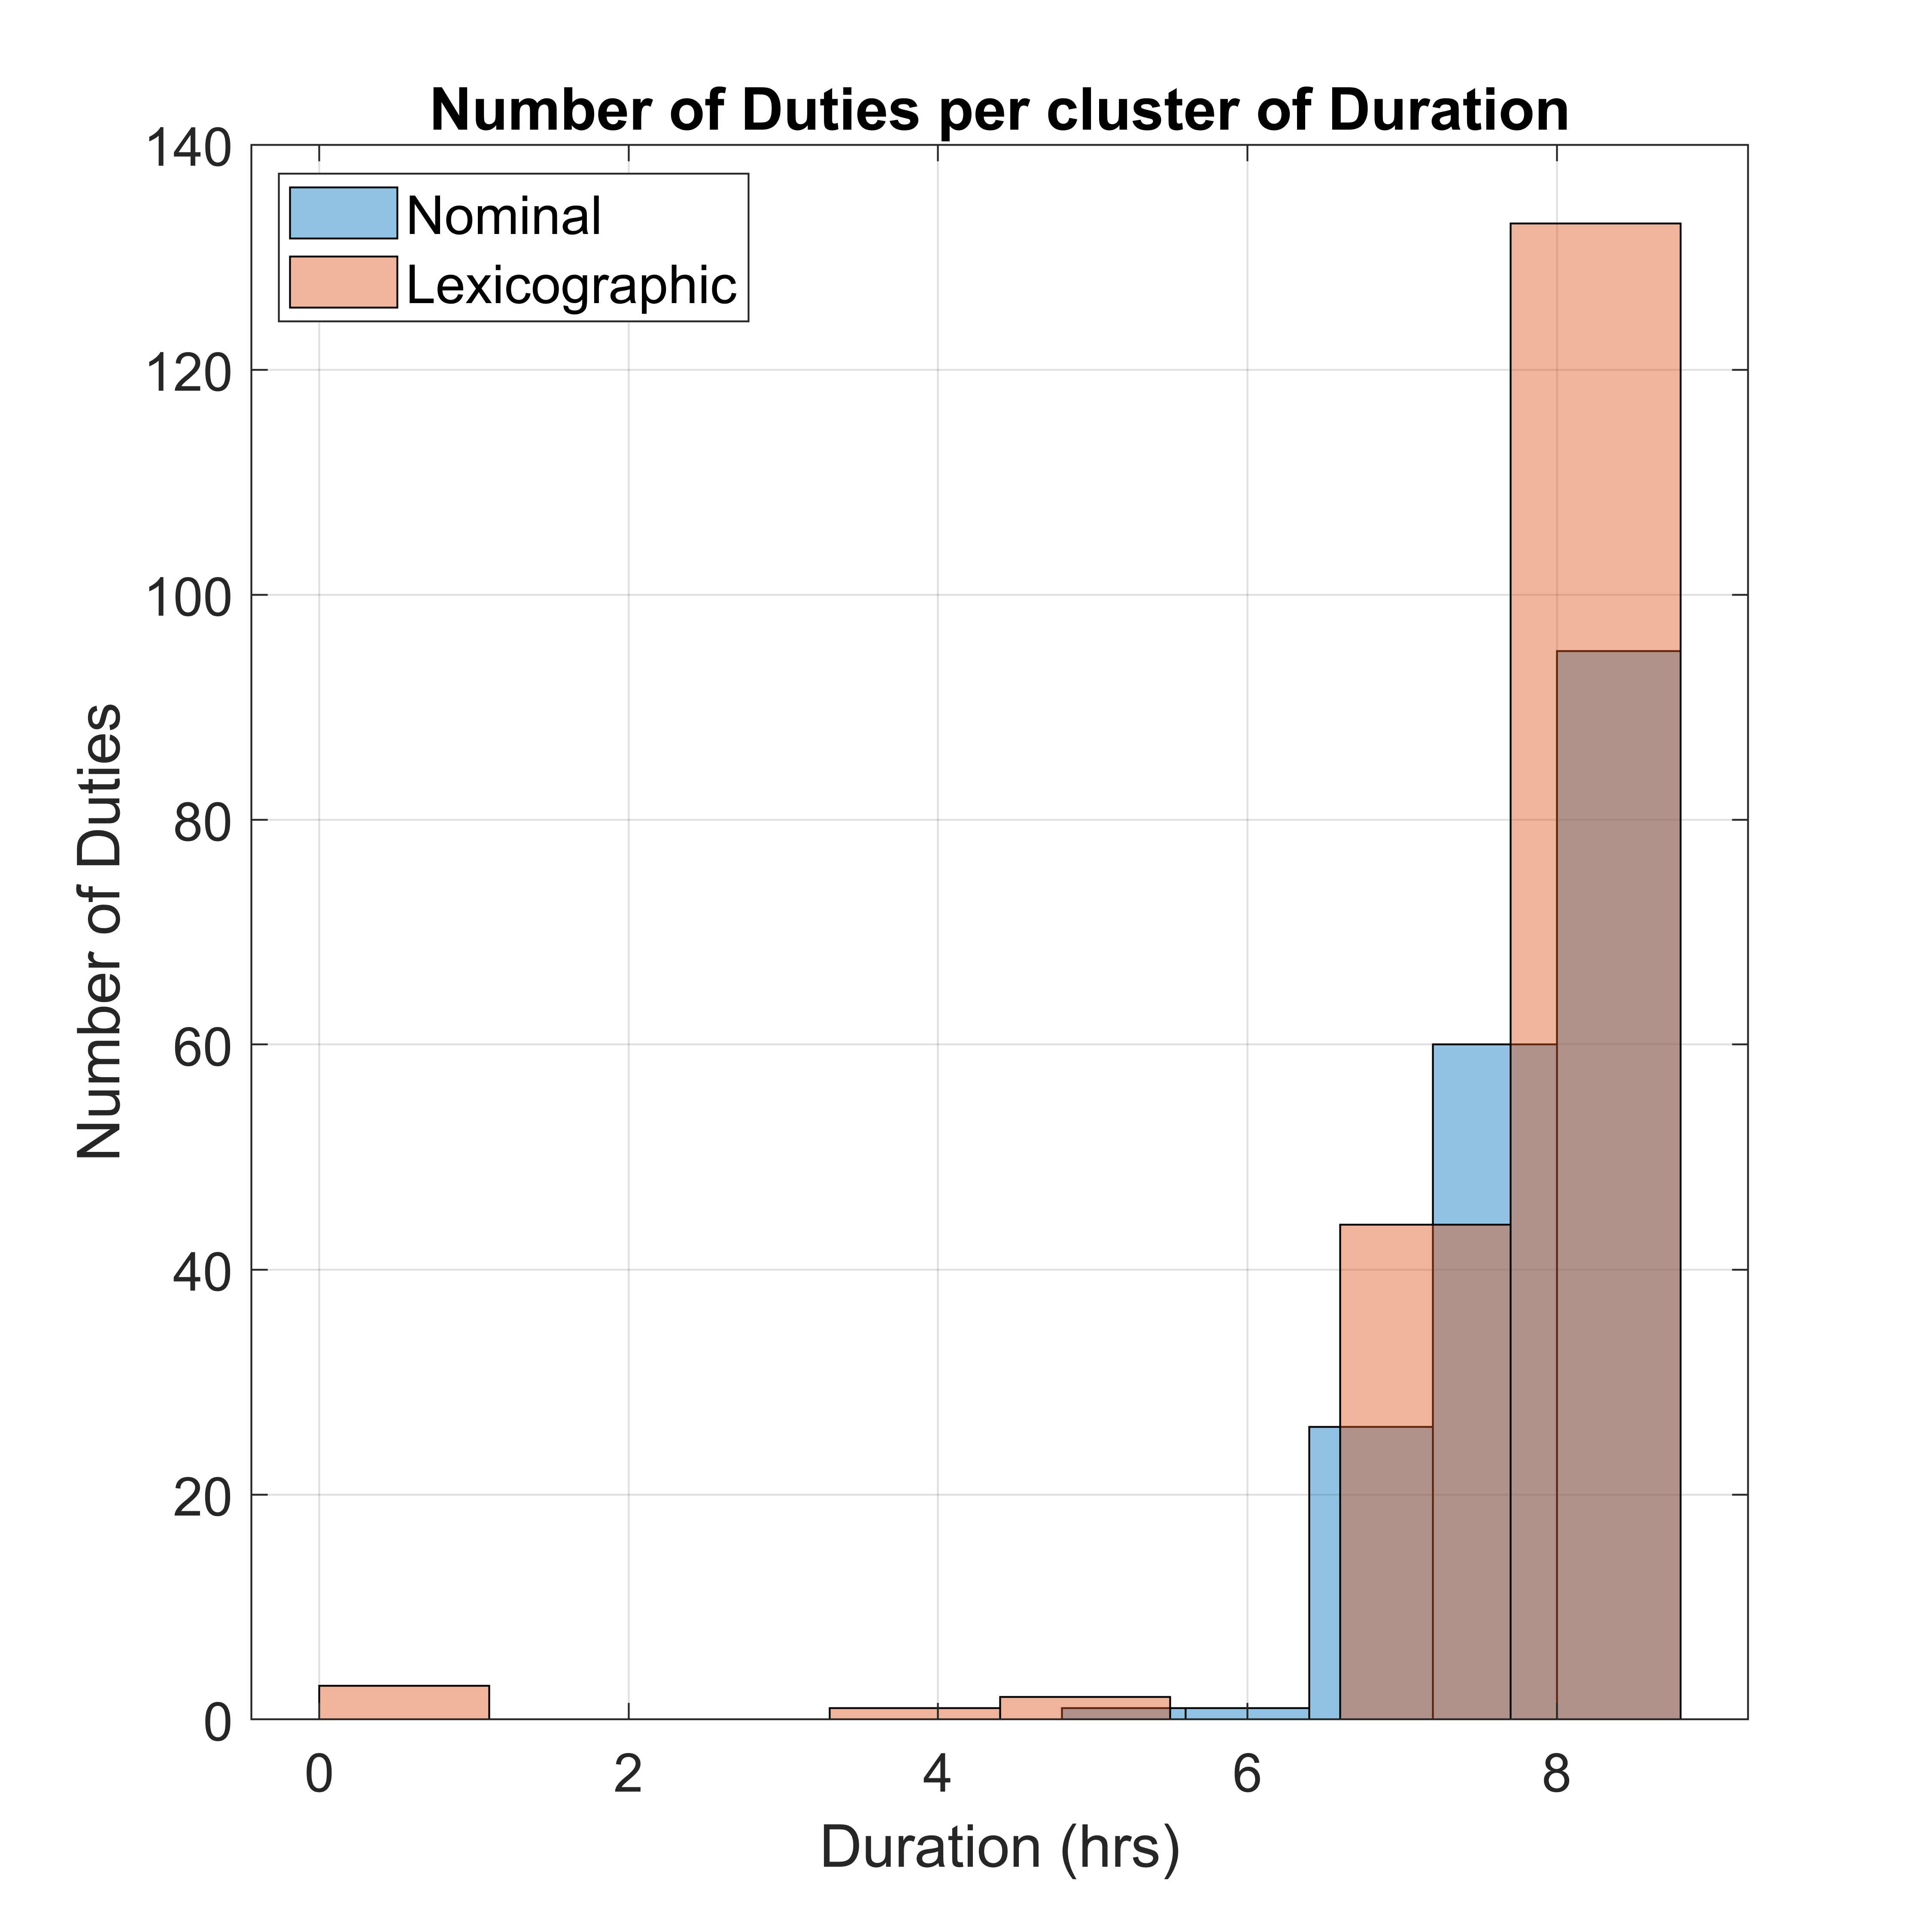
\includegraphics[width=0.46\linewidth]{[3] - chapter/nominal_vs_lexicographic.png}
    }%\end{center}}%end of picture #2
    \qquad
    %picture #2
    \centering
    \subfloat[Table comparing the characteristics of the two schedules.]{\raisebox{9em}{\begin{tabular}{|c|c|c|}
        \hline
        \textbf{Schedule} & \multicolumn{2}{|c|}{ \textbf{Characteristics}} \\
        \hline
         & \texttt{Makespan} &  \texttt{Minimum}  \\
        \hline
        Nominal & 08:25 & 05:15 \\
        \hline
        Lexicographic & 08:25 & 00:00 \\
        \hline
    \end{tabular}}}%
    \caption{Comparison of the Lexicographic and recovered-(i.e. nominal) schedules.}
    \label{fig: Nominal vs Lexicographic.}
\end{figure}

\vspace{\baselineskip}
\noindent
As we can see, the lexicographical schedule maintains the same makespan as the nominal, however is quite more tightly concentrated on duties lasting between 6-7 hours, and also has duties lasting considerably less, even down to duties of zero length.
%%%%%%%%%%%%%%%%%%%%%%% this tell us that then when we appply uncertainty

\vspace{\baselineskip}
\noindent
To determine the robustness of the lexicographic schedule to uncertainty, we apply the \texttt{reduced} and \texttt{augmented} instances for each of the $U:$ $\pm30\%$,$\pm40\%$,$\pm50\%$, and observe the effects each has on this newly generated schedule, in comparison to the previously observed effects on the nominal schedule.

%%%%%%%%%%%%%%%%%%%%%%%%%%%%%%%%%%%%%%%%%%%%%%%%%%%%%%%%%%%%%%%%%%%%%% Table %%%%%%%%%%%%%%%%%%%%%%%%%%%%%%%%%%%%%%%%%%%%%%%


\begin{table}
\small
    \centering 
    \begin{tabular}{|c|c|c|c|c|c|c|c|}
        \hline
        \rowcolor{Gainsboro!90}
        \multicolumn{2}{|c|}{\textbf{Schedule}} & \textbf{LexOpt} & \textbf{Total Time} & \multicolumn{3}{|c|}{ \textbf{Duties (HH:mm)}} & \textbf{Overrun Duties} \\
        \hline
        \multicolumn{4}{|c|}{ }  & \texttt{Makespan} & \texttt{Minimum} & \texttt{Average} &   \\
        \hline
        \multicolumn{2}{|c|}{\textbf{Instance}} &\multicolumn{6}{|c|}{ }\\
        \hline
        \multirow{4}{*}{$U$: $\pm30\%$} & \multirow{2}{*}{\texttt{reduced}} & \cmark & 1,395:54 & 10:49 & 00:00 & 07:37 & 43\\
        \cline{3-8}
         & & \xmark & 1,395:50 & 10:46 & 04:35 & 07:37 & 44\\
        \cline{2-8}
         & \multirow{2}{*}{\texttt{augmented}}& \cmark& 1,456:10 & 10:53 & 00:00 & 07:57 & 58 \\
         \cline{3-8}
         & & \xmark & 1,452:38 & 10:46 & 04:16 & 07:56 & 60\\
        \hline
        \multirow{4}{*}{$U$: $\pm40\%$} &\multirow{2}{*}{\texttt{reduced}}& \cmark& 1,427:18 & 12:16 & 03:38 & 07:47 & 64  \\
         \cline{3-8}
         & & \xmark & 1,416.47 & 11:29 & 04:00 & 07:44 & 66\\
        \cline{2-8}
         &\multirow{2}{*}{\texttt{augmented}}&\cmark & 1,444:57 & 11:45 & 00:00 & 07:53 & 68\\
         \cline{3-8}
         & & \xmark & 1,442:05 & 11:41 & 04:34 & 07:52 & 68\\
        \hline
        \multirow{4}{*}{$U$: $\pm50\%$} &\multirow{2}{*}{\texttt{reduced}}& \cmark& 1,387:40 & 12:15 & 00:00 & 07:34 & 57  \\
         \cline{3-8}
         & & \xmark & 1,386.40 & 12:15 & 03:20 & 07:34 & 58\\
        \cline{2-8}
         &\multirow{2}{*}{\texttt{augmented}}&\cmark & 1,445:08 & 12:22 & 00:00 & 07:53 & 79 \\
         \cline{3-8}
         & & \xmark & 1,445:31 & 12:19 & 03:41 & 07:53 & 79\\
        \hline
    \end{tabular}%
    \medbreak
    \caption{Table compares the Lexicographic\footnote{Represented with (\cmark)} and recovered\footnote{Represented with (\xmark)} disturbed versions of the Nominal schedule. }
    \label{table: Nominal vs Lexicographic}
\end{table}

\vspace{\baselineskip}
\noindent
As we can see from Table \ref{table: Nominal vs Lexicographic}, the Lexicographic schedule performs only marginally better than the nominal schedule in one of the two evaluation criteria. Namely, it performs marginally better in terms of the number of duties overrun since as observed on the final column of the table there are consistently less duties overrun in the lexicographic schedule compared to the nominal. However, it is marginally outperformed in terms of the makespan by the disturbed nominal schedule. 

\vspace{\baselineskip}
\noindent
Taking into consideration the above set of results, one can argue that it is questionable to call the Lexicographic schedule \textbf{more robust} than the nominal one. However, in reality it depends on the scheduler to decide which of the two criteria is of more significance for Royal Mail. Namely, is it more important for Royal Mail, for drivers to have a shorter maximum duty length \textit{L} or would they rather have less duties running longer than the pre-defined threshold. Arguably, a pragmatic approach would conclude that it is considerably more important to have a schedule that ensures that the least amount of duties possible end up crossing the \textit{L'} threshold. That is since the costs that could be incurred from overtime compensation due to a substantial amount of duties overruning are most likely going to be substantially higher compared to a handful of minutes increase in the length of the longest lasting duty (i.e. makespan). Hence, it is our opinion that the Lexicographic schedule can be characterised as more robust due to its lower allowance of duties running very long, despite its longer lasting makespans. 


\subsection*{Minimisation of the Squared Completion Time}
The secondary method that we would like to check, in our quest to enhance the robustness of our nominal schedule is that of the \textit{Minimisation of the Squared Completion Time}. This is a slightly transformed formulation that stems from the Makespan Scheduling formulation of Section \ref{section:Makespan Scheduling-content} of Chapter \ref{chapter: 2-Evaluating Royal Mail Historical Data}. The reasoning behind the choice of this method is two-fold. Firstly, a makespan scheduling based formulation loosely guarantees a well-balanced schedule. This would most likely translate to a schedule where a minimal amount of duties end up overrunning. Moreover, by slightly tweaking the objective function, and instead of minimising the makespan we refocus our formulation towards minimising its square, we will target the longer-lasting duties significantly more. That is because by minimising its square we effectively penalise significantly more the longer lasting duties. This idea stems from the philosophy followed in linear regression. The transformed formulation that we will be applying can be seen below:

%%%%%%%%%%%%%%%%%%%%%%%%%%%%%%%%%%%%%%%%%%%%%%%%%%%%%%%%%%%%%%%%%%%%%%%%%%%%%%% Maths %%%%%%%%%%%%%%%%%%%%%%%%%%%%%%%%%%%%%%%%%%%%%%%%%%%%%%%%%%%%%%%%%%%%%%%%%%%%%%

\vspace{\baselineskip}
\begin{equation}
\label{equation: Makespan Squared Scheduling}
\begin{aligned}
&\text{minimise}
%& & y_{i}  \\ %\todo{why y and and not yi}
& & y^2  \\ 
& \text{subject to}
% & & y_{i} = \sum _{j=1}^n x_{i,j}p_{j}  \;\;\; &\forall \; i \in D\tag{1}\\   
& & y \geq \sum _{j=1}^n x_{i,j}p_{j}  \;\;\; &\forall \; i \in D\\   
& & &\sum _{i=1}^m x_{i,j} = 1 \;\;\; &\forall \; j \in B\\
% & & &\sum _{j=1}^n x_{i,j}p_{j} \leq f_{i}-s_{i} \;\;\; &\forall \; i \in D\\ %{\color{red} we deleted the constraint that involves the length of duty being less than end-start.}
& & & y\geq 0  \\
& & & x_{i,j} \in  \{ 0,1 \} \;\;\; &\forall \; j \in B, \; i \in D\\
\end{aligned}
\end{equation}

\vspace{\baselineskip}
\noindent
The formulation is identical to equation \ref{equation: Makespan Scheduling} of Chapter \ref{chapter: 2-Evaluating Royal Mail Historical Data}, except for the objective function. The objective is to get the \textbf{minimal} possible squared of \textbf{makespan} as opposed to previously simply minimising the makespan.
%%%%%%%%%%%%%%%%%%%%%%%%%%%%%%%%%%%%%%%%%%%%%%%%%%%%%%% Double Figure %%%%%%%%%%%%%%%%%%%%%%%%%%%%%%%%%%%%%%%%%%%%%%%%%%%%%%%%%%%%%%%%%%%%%%%%%%%

\begin{figure}%
    \centering
    \subfloat[Histogram showing the comparison of distributions of block per duty length of the two schedules.]{%\begin{center}
    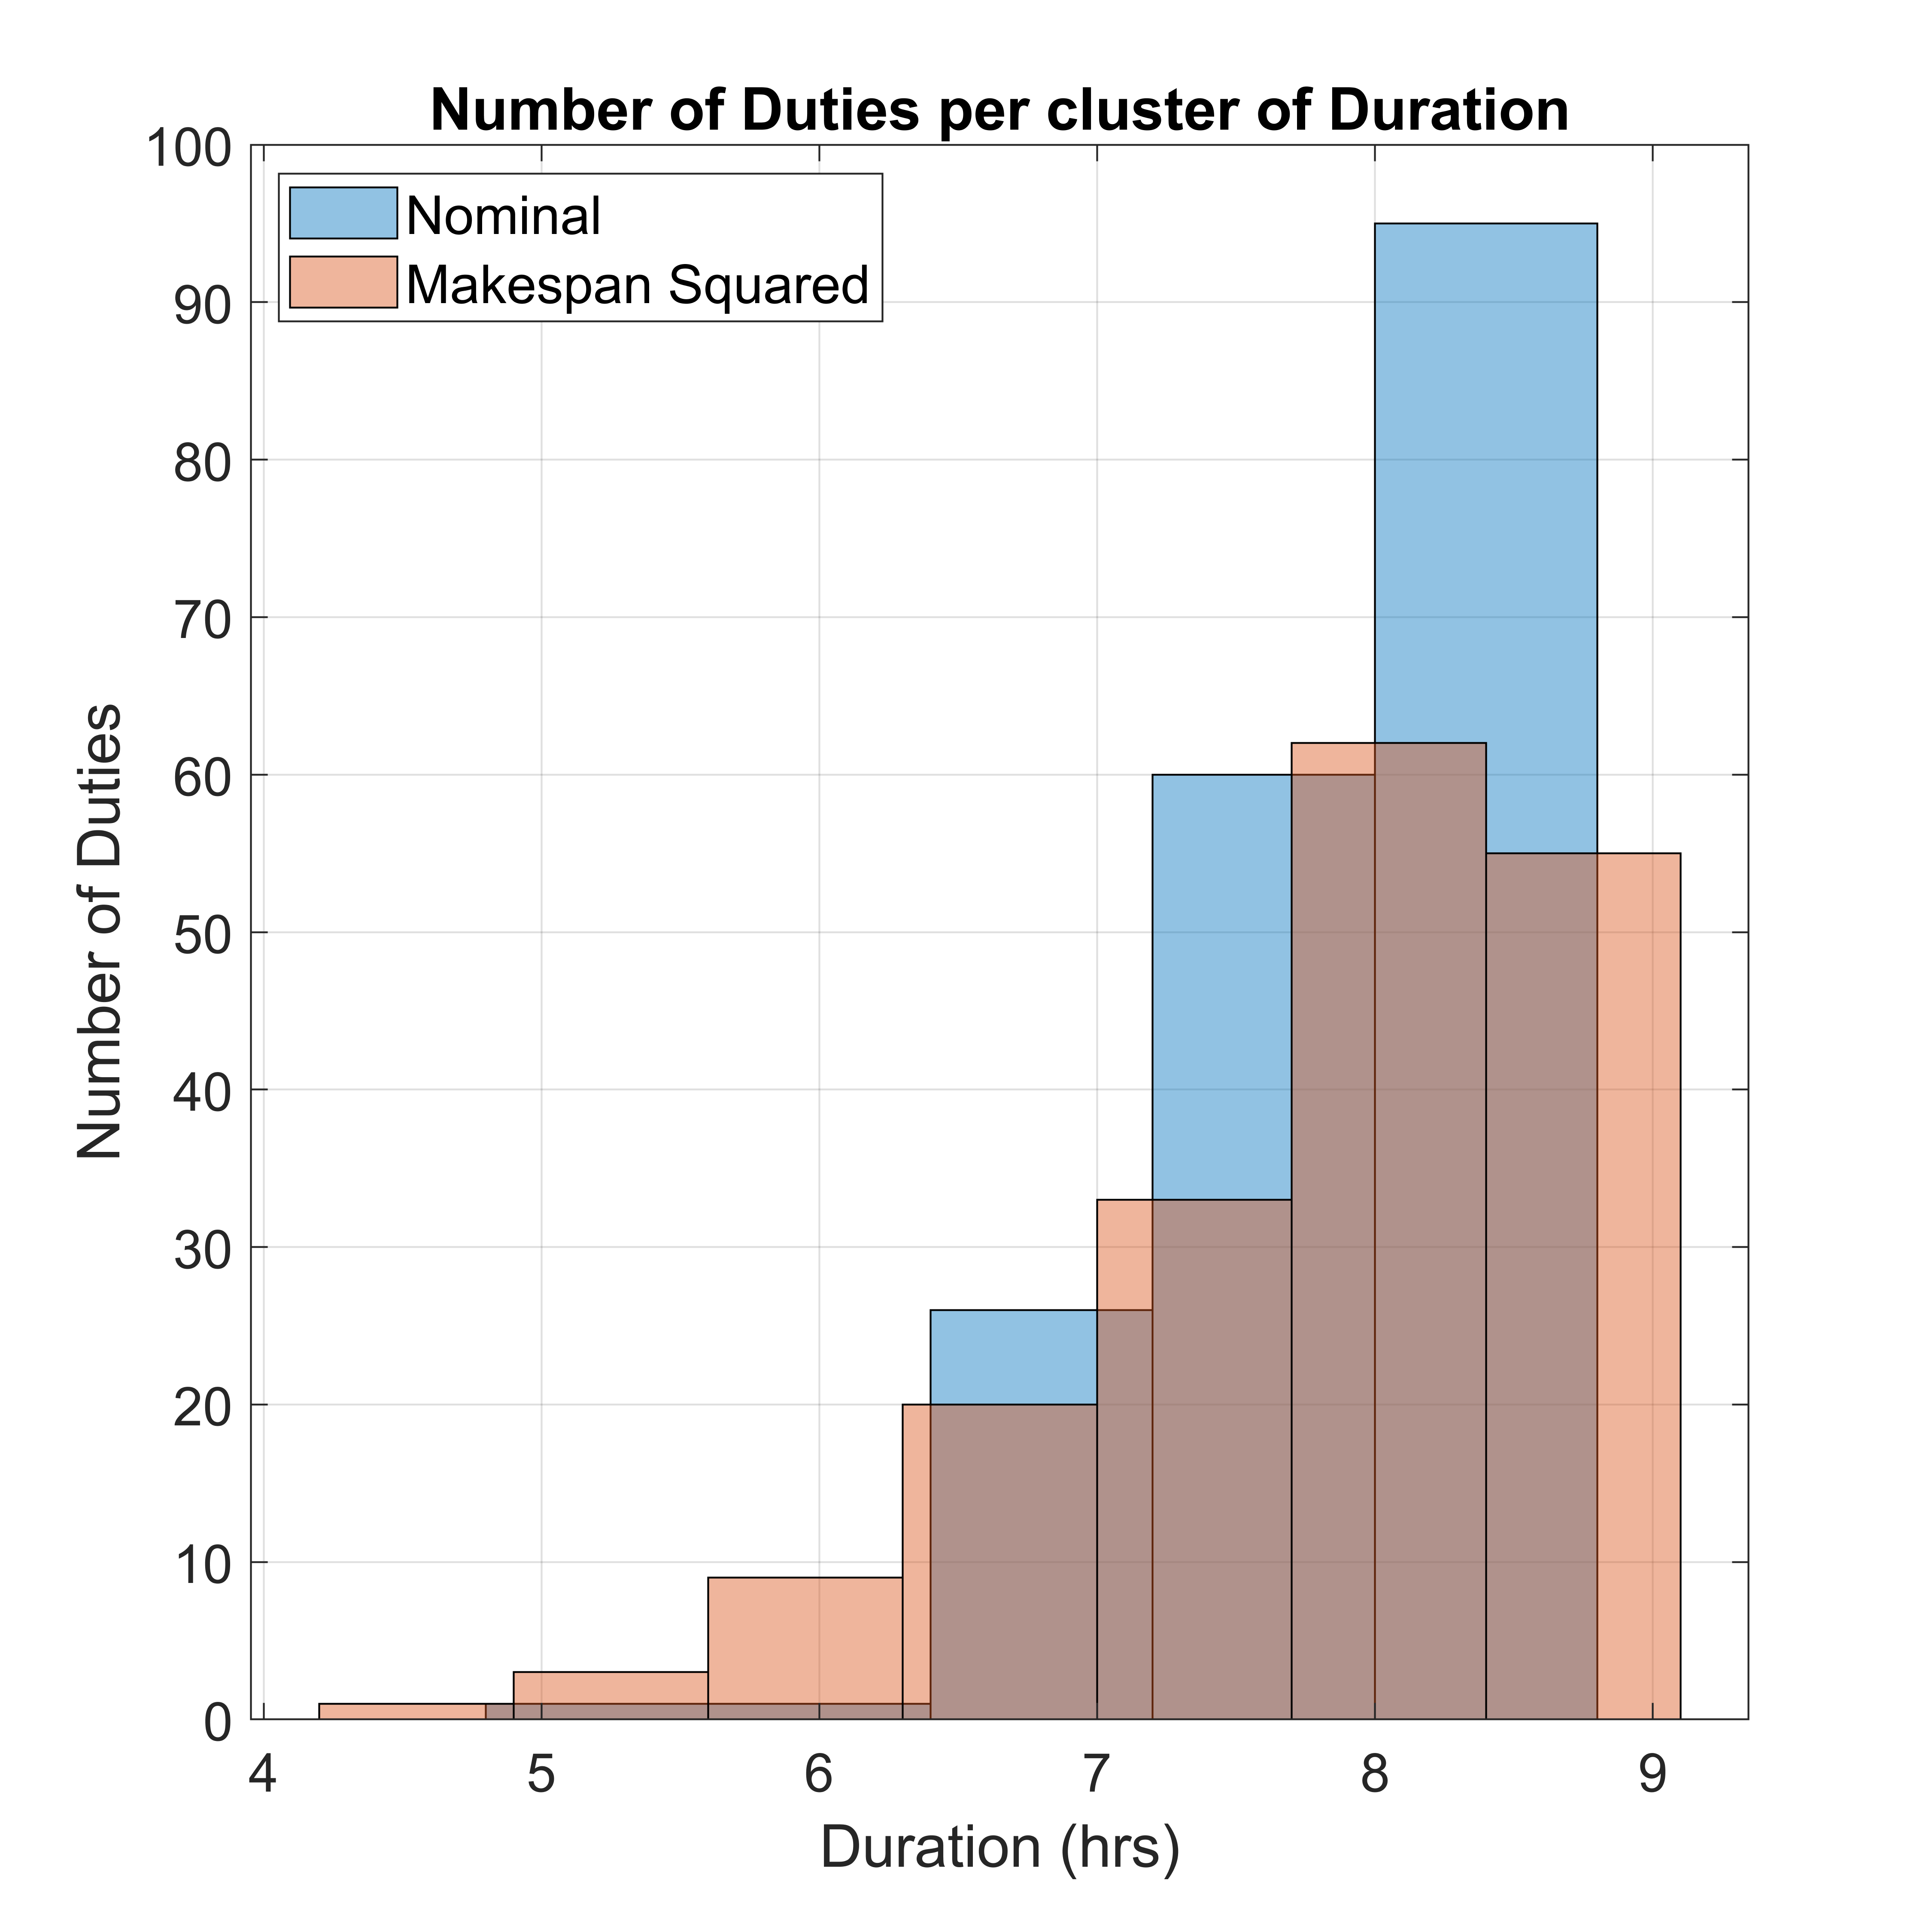
\includegraphics[width=0.46\linewidth]{[3] - chapter/nominal_vs_squared.png}
    }%\end{center}}%end of picture #2
    \qquad
    %picture #2
    \centering
    \subfloat[Table comparing the characteristics of the two schedules.]{\raisebox{9em}{\begin{tabular}{|c|c|c|}
        \hline
        \textbf{Schedule} & \multicolumn{2}{|c|}{ \textbf{Characteristics}} \\
        \hline
         & \texttt{Makespan} &  \texttt{Minimum}  \\
        \hline
        Nominal & 08:25 & 05:15 \\
        \hline
        Makespan Squared & 09:04 & 04:34 \\
        \hline
    \end{tabular}}}%
    \caption{Comparison of the Makespan Squared and Makespan Optimised (nominal) schedules.}
    \label{fig: Nominal vs Squared.}
\end{figure}


\vspace{\baselineskip}
\noindent
As one can determine from Figure \ref{fig: Nominal vs Squared.} the two schedules as expected resemble each other quite a lot, given that they stem from a principally similar formulation. However, we can notice that Makespan Squared model has a slightly longer bandwidth that also contributes to each longer lasting makespan. We subsequently, apply the disturbed instances on it to see its robustness against those uncertainty components, compared to the nominal schedule.

\vspace{\baselineskip}
\noindent
Through a thorough analysis of Table \ref{table: Nominal vs Makespan Squared}, one can determine that the Makespan Squared formulation performs substantially sub-par when compared to the nominal Schedule in both criterion. The makespan is consistently higher, and there are generally more duties that end up overrunning compared to the nominal schedule.

\vspace{\baselineskip}
\noindent
As a result, overall we can conclude that the lexicographically generated schedule is the most robust schedule that makes the least amount of compromise with respect to the minimisation of its Makespan.
%%%%%%%%%%%%%%%%%%%%%%%%%%%%%%%%%%%%%%%%%%%%%%%%%%%%%%%%%%%%%%%%%%%%%% Table %%%%%%%%%%%%%%%%%%%%%%%%%%%%%%%%%%%%%%%%%%%%%%%


\begin{table}
\small
    \centering 
    \begin{tabular}{|c|c|c|c|c|c|c|c|}
        \hline
        \rowcolor{Gainsboro!90}
        \multicolumn{2}{|c|}{\textbf{Schedule}} & \textbf{Squared} & \textbf{Total Time} & \multicolumn{3}{|c|}{ \textbf{Duties (HH:mm)}} & \textbf{Overrun Duties} \\
        \hline
        \multicolumn{4}{|c|}{ }  & \texttt{Makespan} & \texttt{Minimum} & \texttt{Average} &   \\
        \hline
        \multicolumn{2}{|c|}{\textbf{Instance}} &\multicolumn{6}{|c|}{ }\\
        \hline
        \multirow{4}{*}{$U$: $\pm30\%$} & \multirow{2}{*}{\texttt{reduced}} & \cmark & 1,405:43 & 11:19 & 03:57 & 07:40 & 83\\
        \cline{3-8}
         & & \xmark & 1,395:50 & 10:46 & 04:35 & 07:37 & 44\\
        \cline{2-8}
         & \multirow{2}{*}{\texttt{augmented}}& \cmark& 1,457:31 & 11:36 & 04:49 & 07:57 & 73 \\
         \cline{3-8}
         & & \xmark & 1,452:38 & 10:46 & 04:16 & 07:56 & 60\\
        \hline
        \multirow{4}{*}{$U$: $\pm40\%$} &\multirow{2}{*}{\texttt{reduced}}& \cmark& 1,427:18 & 12:16 & 03:38 & 07:47 & 101  \\
         \cline{3-8}
         & & \xmark & 1,416.47 & 11:29 & 04:00 & 07:44 & 66\\
        \cline{2-8}
         &\multirow{2}{*}{\texttt{augmented}}&\cmark & 1,456:17 & 12:41 & 03:31 & 07:57 & 97\\
         \cline{3-8}
         & & \xmark & 1,442:05 & 11:41 & 04:34 & 07:52 & 68\\
        \hline
        \multirow{4}{*}{$U$: $\pm50\%$} &\multirow{2}{*}{\texttt{reduced}}& \cmark& 1,392:27 & 12:54 & 03:23 & 07:36 & 99  \\
         \cline{3-8}
         & & \xmark & 1,386.40 & 12:15 & 03:20 & 07:34 & 58\\
        \cline{2-8}
         &\multirow{2}{*}{\texttt{augmented}}&\cmark & 1,446:46 & 13:05 & 03:37 & 07:54 & 88 \\
         \cline{3-8}
         & & \xmark & 1,445:31 & 12:19 & 03:41 & 07:53 & 79\\
        \hline
    \end{tabular}%
    \medbreak
    \caption{Table compares the Makespan Squared\footnote{Represented with (\cmark)} and recovered\footnote{Represented with (\xmark)} disturbed versions of the Nominal schedule. }
    \label{table: Nominal vs Makespan Squared}
\end{table}
\vspace*{3in}
\vspace{\baselineskip}